\documentclass[aspectratio=169,usenames, dvipsnames, 11pt]{beamer}

% theme determines the design in terms of shapes in the presentation
\usetheme{madrid}
% themes are:
% AnnArbor
% Antibes
% Bergen
% Berkeley
% Berlin
% Boadilla
% CambridgeUS
% Copenhagen
% Darmstadt
% Dresden
% Frankfurt
% Freiburg
% Goettingen
% Hannover
% Ilmenau
% JuanLesPins
% Luebeck
% Madrid
% Malmoe
% Marburg
% Montpellier
% PaloAlto
% Pittsburgh
% Rochester
% Singapore
% Szeged
% Warsaw
%
% from: https://www.namsu.de/latex/themes/uebersicht_beamer.html

% combining inner and outer themes
%\useoutertheme{infolines}
% available outer themes
% from: https://www.namsu.de/latex/themes/outer.html
% infolines
% miniframes
% shadow
% sidebar
% smoothbars
% smoothtree
% split
% tree

\useinnertheme{rectangles}
% available inner themes
% from: https://www.namsu.de/latex/themes/inner.html
% circles
% rounded
% rectangles

% explicitly prevent rounded blocks and shadows
%\setbeamertemplate{blocks}[rounded][shadow=true]
\setbeamertemplate{blocks}[default]

% title page
\setbeamertemplate{title page}[default][colsep=-4bp,rounded=false]

% The color theme defines the color used for a theme.
% One can set all custom colors, or just apply one color to the structrue of the presentation

% own color
\definecolor{mycolor}{rgb}{0.0,0.35,0.6}
\definecolor{lightgray}{RGB}{212,212,212}
\definecolor{mgray}{RGB}{132,132,132}
\definecolor{orange}{RGB}{230,113,43}
\definecolor{purpel}{rgb}{0.5,0,0.5}
\definecolor{grun}{rgb}{0.0,0.4,0.0}
\definecolor{blau}{rgb}{0.1,0.3,0.5}

\usecolortheme[named=mycolor]{structure}

% Color names from xcolor package can be used
% from: https://en.wikibooks.org/wiki/LaTeX/Colors#Predefined_colors
%	Apricot 	  	  	Aquamarine
%	Bittersweet 	  	Black
%	Blue 	  	  	  	BlueGreen
%	BlueViolet 	  	  	BrickRed
%	Brown 	  	  	  	BurntOrange
%	CadetBlue 	  	  	CarnationPink
%	Cerulean 	  	  	CornflowerBlue
%	Cyan 	  	  	  	Dandelion
%	DarkOrchid 	  	  	Emerald
%	ForestGreen 	  	Fuchsia
%	Goldenrod 	  	  	Gray
%	Green 	  	  	  	GreenYellow
%	JungleGreen 	  	Lavender
%	LimeGreen 	  	  	Magenta
%	Mahogany 	  	  	Maroon
%	Melon 	  	  	  	MidnightBlue
%	Mulberry 	  	  	NavyBlue
%	OliveGreen 	  	  	Orange
%	OrangeRed 	  	  	Orchid
%	Peach 	  	  	  	Periwinkle
%	PineGreen 	  	  	Plum
%	ProcessBlue 	  	Purple
%	RawSienna 	  	  	Red
%	RedOrange 	  	  	RedViolet
%	Rhodamine 	  	  	RoyalBlue
%	RoyalPurple 	  	RubineRed
%	Salmon 	  	  	  	SeaGreen
%	Sepia 	  	  	  	SkyBlue
%	SpringGreen 	  	Tan
%	TealBlue 	  	  	Thistle
%	Turquoise 	  	  	Violet
%	VioletRed 	  	  	White
%	WildStrawberry 	  	Yellow
%	YellowGreen 	  	YellowOrange

% Using tikz for charts, diagrams
\usepackage{tikz}
% for relative positioning
\usetikzlibrary{positioning}

\usepackage[utf8]{inputenc}
\usepackage{PTSans}
\usepackage{inconsolata}
\usepackage{listings}
\lstset{
	basicstyle=\ttfamily\footnotesize,
	language=bash,
	showstringspaces=false,	% do not emphasize spaces in strings
	tabsize=4,				% number of spaces of a TAB
	mathescape=false,		% Dont escape to math mode with $
	escapechar=§,			% escape to latex with §...§
	upquote=false,			% upright quotes (aus lassen, gibt Fehler)
	columns=fixed,			% nice spacing
	backgroundcolor=\color{lightgray}, % background color
	stringstyle=\color{purpel},
	commentstyle=\color{grun},
	xleftmargin=0.1cm,
	frame=l,
	rulecolor=\color{mgray},
	framerule=2pt,
	keywordstyle=\color{blau},
	morekeywords={FROM, ENV, ADD, COPY, RUN, CMD, ENTRYPOINT, ARG, LABEL, WORKDIR}
}

% Some custom inline text decoration
\newcommand{\hervor}[1]{\textcolor{orange}{#1}}
\newcommand{\codi}[1]{\colorbox{lightgray}{\texttt{\footnotesize#1}}} 
\newcommand{\myhref}[2]{\href{#1}{\textcolor{mycolor}{\underline{#2}}}} 
\newcommand{\bs}{\textbackslash}

\newcommand{\sectionslide}[1]{
	{
		\setbeamercolor{background canvas}{bg=mycolor}
		\begin{frame}[noframenumbering]
			\thispagestyle{empty}
			\textcolor{white}{\Huge #1}
		\end{frame}
	}
	
}
% remove navigation symbols
\beamertemplatenavigationsymbolsempty

% Titlepage data
\title{Virtualization with Containers and Kubernetes}
\author{Andreas Roth}
\date{09.06.2021}
\subtitle{Introduction with a focus on Docker}
\institute{Training}

% start the document
\begin{document}

\begin{frame}
	\titlepage
\end{frame}

\begin{frame}[noframenumbering]
	\frametitle{Contents}
	\tableofcontents
\end{frame}

\section{Virtualization}
\sectionslide{Virtualization}
\begin{frame}
	\frametitle{Virtualization}
	\begin{columns}
		\column{.5\textwidth}		
		
		Classical view of \textbf{a computer} running \textbf{an operating system}, running \textbf{a program}.
		\vspace{0.5cm}
		\begin{itemize}
			\item OS is in full control of the hardware
			\item A program runs with lower privilege
			\item OS assigns resources to program
		\end{itemize}
		\vspace{0.5cm}
		OS acts as a \textbf{supervisor} for programs.
		
		\column{.5\textwidth}
		\centering
		\begin{tikzpicture}
			\node[] (comp) at (0,0) {
\includegraphics[width=5.6cm]{pics/computer.png}};
			\node[] (os) [above=0cm of comp] {
\includegraphics[width=5.6cm]{pics/os_prog.png}};
		\end{tikzpicture}
		
	\end{columns}	
\end{frame}

\begin{frame}
	\frametitle{Virtualization}
	\begin{columns}
		\column{.6\textwidth}
		\begin{block}{Virtual Machine Monitor\footnotemark[1] (\textbf{Hypervisor})}
			\begin{enumerate}
				\item provides environment essentially identical to original machine
				\item in full control of system resources
				\item Programs run with minimal speed decreases in this environment
			\end{enumerate}
		\end{block}
	
		\begin{block}{Virtual Machine\footnotemark[1]}
			The environment for \textbf{programs} to run in, with a \textbf{Hypervisor} present, is called a \textbf{Virtual Machine}.
		\end{block}
		
		\column{.4\textwidth}
		\centering
		\begin{tikzpicture}
			\node[] (comp) at (0,0) {
\includegraphics[width=4.6cm]{pics/computer.png}};
			\node[] (hyp) [above=-0.2cm of comp] {
\includegraphics[width=4.6cm]{pics/hypervisor.png}};
			\node[] (os) [above=-0.2cm of hyp] {
\includegraphics[width=4.6cm]{pics/os_prog.png}};
		\end{tikzpicture}
	\end{columns}
	\footnotetext[1]{\tiny Popek G.J., Goldberg R. P. \textit{Formal Requirements for Virtualizable Third Generation Architectures}, Commmunications of the ACM, Volume 7 (17), 1974}
	
\end{frame}

\section{Containers}
\sectionslide{Containers}
\begin{frame}
	\frametitle{"Containerization" - A kind of virtualization...}
	
	\begin{columns}
		\column{.55\textwidth}
			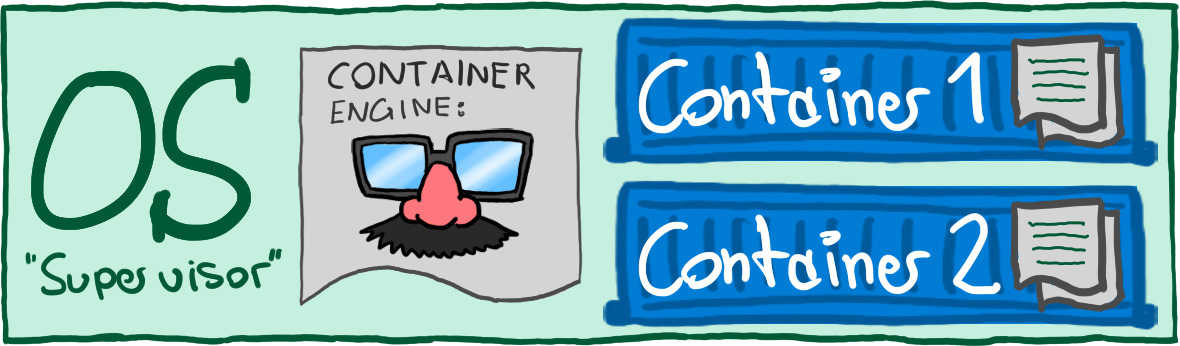
\includegraphics[width=.95\textwidth]{pics/os_cont.png}
			
		\column{.45\textwidth}
			\begin{block}{OS-level virtualization\footnotemark[1]}
				OS allows multiple instances of isolated user spaces (\textbf{containers}) to run applications in. They all share the OS Kernel.
			\end{block}
	\end{columns}

	\begin{columns}
		\column{.3\textwidth}
			
\includegraphics[width=\textwidth]{pics/computer.png}
		\column{.7\textwidth}
			\begin{itemize}
				\item Processes inside the container cannot see anything outside (processes, files, ...). Physically, they are processes running on the same OS Kernel, however.
				\item There is no need for a virtualization layer below the Kernel to run containers, although there can be one!
				\item A \hervor{container engine} or \hervor{runtime} manages the containers
			\end{itemize}
	\end{columns}
	
	\footnotetext[1]{\tiny\textit{OS-level Virtualization}, Wikipedia 2021, \href{https://en.wikipedia.org/wiki/OS-level\_virtualization}{https://en.wikipedia.org/wiki/OS-level\_virtualization}}
\end{frame}

\begin{frame}
	\frametitle{Containers}
	\begin{columns}
		\column{.45\textwidth}
		\begin{tikzpicture}
			\node[] (container) at (0,0) {
\includegraphics[width=.9\textwidth]{pics/container_large.png}};
			\node[] (image) [below=1cm of container] {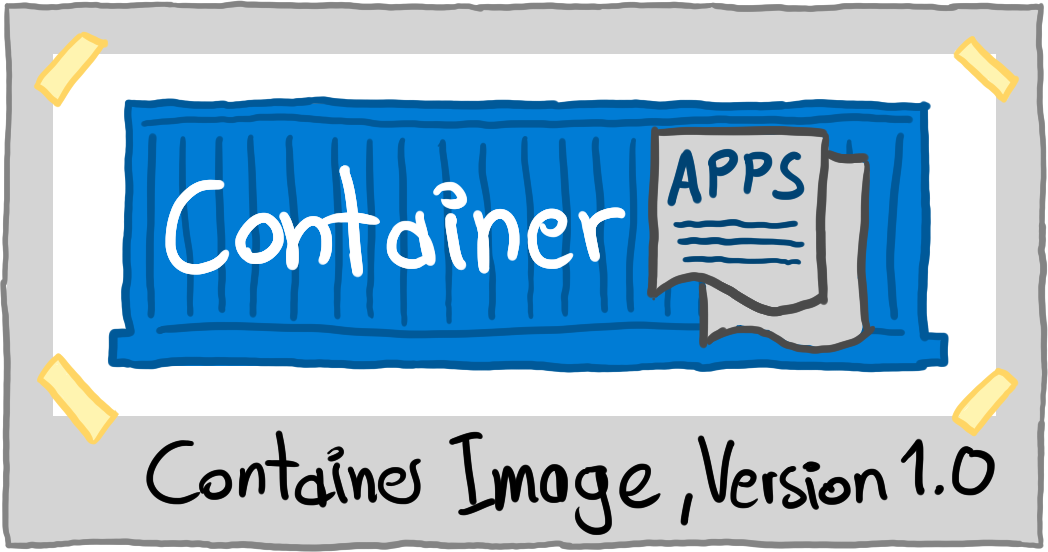
\includegraphics[width=.9\textwidth]{pics/container_image.png}};
			\draw[->, draw=mycolor, line width=5pt] (container)--(image);
		\end{tikzpicture}
		\column{.55\textwidth}
			\textbf{\Large Why?}
			\begin{itemize}
				\item Bundle up an application \hervor{with all its dependencies!}
				\item More \hervor{lightweight and portable} than a virtual machine
			\end{itemize}
		
			\vspace{.25cm}\textbf{\Large How?}
			\begin{itemize}
				\item Containers can be shipped as images (distribution infrastructure depends on system / engine)
				\item Who runs a container based on my image can be sure to have a \hervor{functionally identical environment}, independent of application type
			\end{itemize}
			
	\end{columns}
\end{frame}

\begin{frame}
	\frametitle{How to make containers?}
	\centering
	\textbf{Advanced use of Linux features!}
	\vspace{.5cm}\begin{columns}
		\column{.5\textwidth}
			\hervor{\Large namespaces}
			\begin{itemize}
				\item Limit what a process can \hervor{see}
				\item Change filesystem root with \codi{chroot}
				\item Change apparent \codi{pid}s
				\item ...
			\end{itemize}
		\column{.5\textwidth}
			\hervor{\Large cgroups}
			\begin{itemize}
				\item Limit what a process can \hervor{use}
				\item Hierarchical definition tree to assign quantities of memory, cpu cores, ... to processes and groups of processes
			\end{itemize}
	\end{columns}
	
	\centering
	\vspace{.5cm}Definitely watch those talks:
	\small
	\begin{itemize}
		\item Containers from scratch (Liz Rice, 2018): \myhref{https://www.youtube.com/watch?v=8fi7uSYlOdc}{https://www.youtube.com/watch?v=8fi7uSYlOdc}
		\item Namespaces, cgroups and beyond: What are containers made from? (Jérôme Petazzoni, 2015): \myhref{https://www.youtube.com/watch?v=sK5i-N34im8}{https://www.youtube.com/watch?v=sK5i-N34im8}
	\end{itemize}
	
	
\end{frame}

\begin{frame}
	\frametitle{Container runtimes / engines}
	
	\centering
	There are / might be several software layers between the user interacting with a \textbf{container engine} and the \textbf{runtime} that actually runs containers.
	
	\vspace{.3cm}\begin{columns}[t]
		\column{0.5\textwidth}
		Based on Linux namespaces and cgroups:
		\begin{itemize}
			\item \myhref{https://linuxcontainers.org/}{LXC}
			\item \myhref{https://www.docker.com/}{Docker} (Docker engine, containerd)
			\item \myhref{https://podman.io/}{Podman}
		\end{itemize}
	
		\column{.5\textwidth}
		Other mechanisms / systems:
		\begin{itemize}
			\item \myhref{https://docs.freebsd.org/en/books/arch-handbook/jail/}{FreeBSD Jail} (Unix)
			\item \myhref{https://docs.oracle.com/cd/E36784\_01/html/E36848/zones.intro-1.html\#scrolltoc}{Solaris Zones} (Unix)
			\item \myhref{https://docs.microsoft.com/en-us/virtualization/windowscontainers/quick-start/set-up-environment?tabs=Windows-Server}{Windows Containers}
		\end{itemize}
	\end{columns}

	
\end{frame}



\section{Docker}
\sectionslide{Docker}
\begin{frame}
	\frametitle{Docker}
	
	\begin{columns}
		\column{.55\textwidth}
		\begin{itemize}
			\item Runtime and engine
			\item Building / managing of images / containers
			\item Distribution of images (Docker Hub)
			\item Interface to Windows and MacOS, different mechanisms
			\item (Orchestration of containers) swarm, \codi{docker-compose}
			\item Docker engine exists as open source, Docker Desktop and Docker Hub are developed by \myhref{https://www.docker.com/company}{Docker Inc.}
		\end{itemize}
		\column{.45\textwidth}
		\textbf{Docker is the most relevant container tool for us.}
		
		\vspace{.2cm}We will take a short tour of the most important \hervor{Docker concepts}:
		\begin{itemize}
			\item Running containers
			\item Building images with \codi{Dockerfile}s
			\item Docker registries (\myhref{https://hub.docker.com/}{Docker Hub}, company self-hosting solutions)
			\item Pushing / pulling images
			\item Docker volumes
		\end{itemize}
	\end{columns}
	
\end{frame}

\begin{frame}
	\frametitle{Code-along exercises}
	
	\centering
	
\includegraphics[width=3cm]{pics/codealong.png}
	
	\begin{itemize}
		\item Feel free to try out the commands presented on the next slides during the training!
		\item You need a \myhref{https://www.docker.com/products/docker-desktop}{Docker Desktop} installation (or \myhref{https://hub.docker.com/search?offering=community\&operating\_system=linux\&q=\&type=edition}{Docker Engine on Linux})
		\item As a preparation, clone  \myhref{https://github.com/scherbertlemon/docker-training}{github.com/scherbertlemon/docker-training}
	\end{itemize}
\end{frame}

\begin{frame}
	\frametitle{Container registries}
	\begin{block}{Container registries}
		... where prepared container images come from, if you do not build them based on your host system. They are usually organised in versioned image repositories.
	\end{block}
	\vspace{0.25cm}\begin{columns}[t]
		\column{.6\textwidth}
		\myhref{https://hub.docker.com}{Docker Hub} hosted by Docker Inc.
		\begin{itemize}
			\item Open registry where you can store your images in \textbf{repositories}
			\item Public repositories are free of charge
			\item Many \myhref{https://hub.docker.com/search?q=\&type=image\&image\_filter=official}{officially curated images}
		\end{itemize}
		
		\column{.4\textwidth}
		\myhref{}{Your company solution here}
		\begin{itemize}
			\item you might want to host your own registry
		\end{itemize}
	\end{columns}
    \vspace{0.5cm}\begin{itemize}
		\item Connect to a registry with \codi{docker login <url>}. If no URL, Docker Hub is the default.
		\item Generate an \hervor{Access Token} if possible and use it for login instead of your password.
	\end{itemize}
	
\end{frame}

\begin{frame}
	\frametitle{Images and Containers}
	\begin{columns}
		\column{.47\textwidth}
		\centering
			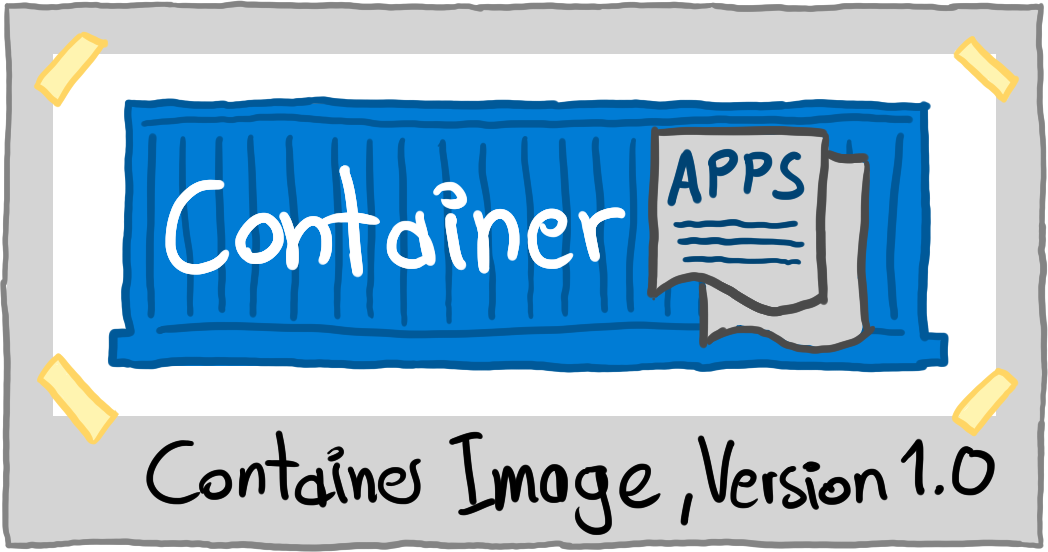
\includegraphics[width=.75\textwidth]{pics/container_image.png}
			
		\column{.47\textwidth}
		\centering
			
\includegraphics[width=.75\textwidth]{pics/container_large.png}
			
	\end{columns}
	\begin{columns}[t]
		\column{.47\textwidth}
		\centering
		\begin{block}{Image}
			Read only content of a container, e.g. file system, environment variables, metadata
		\end{block}
		\begin{itemize}
			\item Organized in \hervor{layers} ("differences")
			\item We usually \hervor{pull / push} images from / to \textbf{container registries}
		\end{itemize}
		
		\column{.47\textwidth}
		\centering
		\begin{block}{Container}
			Extracted image content plus writable layer, that can be run on the host OS.
		\end{block}
		\begin{itemize}
			\item We usually \hervor{run} processes in a container
			\item Changes to the file system exist as long as the container is not stopped and removed
		\end{itemize}
	\end{columns}
\end{frame}

\begin{frame}[fragile]
	\frametitle{Images and Containers}
	\begin{columns}
		\column{.47\textwidth}
		\centering
		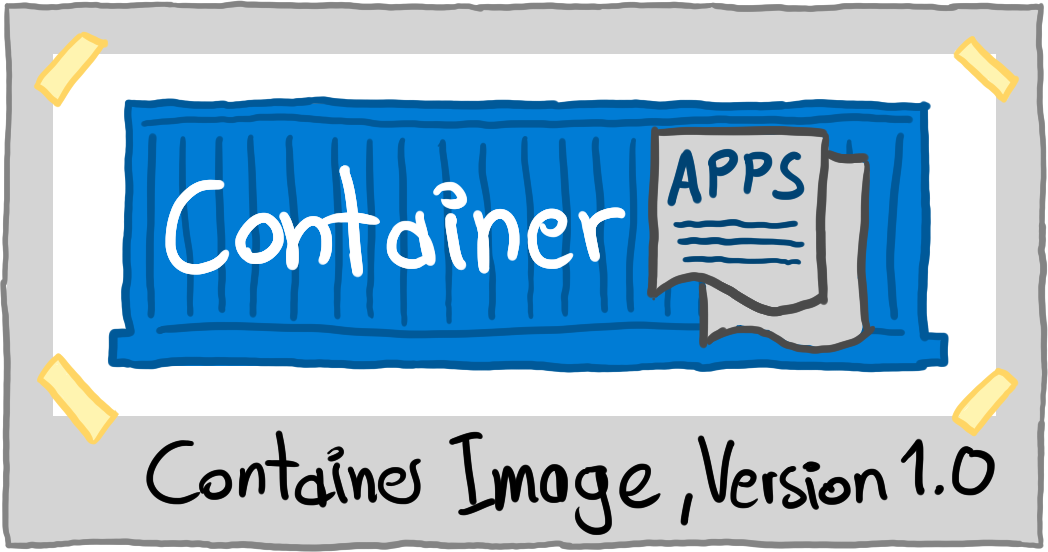
\includegraphics[width=.75\textwidth]{pics/container_image.png}
		
		\column{.47\textwidth}
		\centering
		
\includegraphics[width=.75\textwidth]{pics/container_large.png}
		
	\end{columns}
	\begin{columns}[t]
		\column{.47\textwidth}
		\begin{lstlisting}
# get the offical ubuntu image
docker pull ubuntu:focal
# check the local images
docker image ls
# check the properties of this image
docker image inspect ubuntu:focal
# remove the local image
docker image rm ubuntu:focal
		\end{lstlisting}
		
		\column{.5\textwidth}
		\begin{lstlisting}
# get an interactive shell in ubuntu
docker run -it --name ubu ubuntu:focal
# check the list of containers
docker container ls --all
# check the properties of ubu container
docker container inspect ubu
# remove stopped container
docker container rm ubu
		\end{lstlisting}
	\end{columns}
\end{frame}


\begin{frame}[fragile]
	\frametitle{Building images with Dockerfiles}
	
	\begin{columns}
		\column{.45\textwidth}
		\begin{lstlisting}
FROM ubuntu:focal

LABEL maintainer="someone"

ENV TZ=Europe/Berlin

RUN apt update \
	&& apt install \
	tzdata \
	--yes --no-install-recommends \
	&& rm -rf /var/lib/apt/lists/*

WORKDIR	/wdir
# goes to wdir
COPY localfile.txt .

ENTRYPOINT [ "date" ]
		\end{lstlisting}
		
		\column{.55\textwidth}
		\textbf{Example that prints the time when run}
		\begin{block}{Dockerfile}
			... a recipe to perform certain tasks starting from an image, controlled by \textbf{directives}, to create a new, modified image.
		\end{block}
		\begin{itemize}
			\item find this Dockerfile in \codi{dockerfiles/time}
			\item \myhref{https://docs.docker.com/engine/reference/builder/}{Dockerfile reference}
			\item \myhref{https://docs.docker.com/develop/develop-images/dockerfile\_best-practices/}{Best practises}
			\item Directives: \codi{FROM}, \codi{ENV}, \codi{RUN}, \codi{COPY}, \codi{ENTRYPOINT}, \codi{CMD}
		\end{itemize}

	\end{columns}
\end{frame}

\begin{frame}[fragile]
	\frametitle{Building images with Dockerfiles}
	
	\begin{columns}
		\column{.45\textwidth}
		\begin{lstlisting}
FROM ubuntu:focal

LABEL maintainer="Someone"

ENV TZ=Europe/Berlin

RUN apt update \
	&& apt install \
	tzdata \
	--yes --no-install-recommends \
	&& rm -rf /var/lib/apt/lists/*

WORKDIR	/wdir
# goes to wdir
COPY localfile.txt .

ENTRYPOINT [ "date" ]
		\end{lstlisting}
	
		\column{.55\textwidth}
		\textbf{Example that prints the time when run}
		\begin{lstlisting}
# build an image from Dockerfile in current
# folder
$ docker build -t time:0.1 .
# run it as a container
$ docker run --rm time:0.1
Sun May 30 19:24:10 CEST 2021
# give an argument to date, UTC time
$ docker run --rm time:0.1 -u
Sun May 30 17:24:50 UTC 2021
		\end{lstlisting}
	
	\begin{itemize}
		\item tag/name the image with \codi{name:version}
		\item \codi{.} indicates the \hervor{build context} (current folder)
		\item \codi{--rm} deletes the container after it has stopped running
	\end{itemize}
	\end{columns}
\end{frame}


\begin{frame}[fragile]
	\frametitle{Building a more complex Dockerfile}
	\begin{block}{Simple greeting app}
		\begin{itemize}
			\item We install \myhref{https://repo.anaconda.com/miniconda/Miniconda3-latest-Linux-x86\_64.sh}{miniconda} into our container.
			\item We create a Python environment with \codi{requirements.txt} in \codi{/pysource/env}
			\item We run the \codi{flask} app defined in \codi{greeting.py} in that environment
		\end{itemize}
	\end{block}

	\vspace{-.5cm}\begin{columns}[t]
		\column{.62\textwidth}
		\begin{itemize}
			\item navigate to \codi{dockerfiles/greeting/0.1}
			\item look at the Dockerfile
			\item build\&run it with
		\end{itemize}
		\begin{lstlisting}
docker build -t greeting:0.1 .
docker run --rm -it -p 5000:5000 greeting:0.1
		\end{lstlisting}
		\begin{itemize}
			\item Open your browser at \myhref{http://localhost:5000}{\codi{localhost:5000/hello/yourname}}
		\end{itemize}
		
		
		\column{.38\textwidth}
		\begin{itemize}
			\item \codi{-p host:container} publishes ports from container to host.
			\item Storage is just \hervor{in memory}: when app is restarted, counter is reset
		\end{itemize}
	\end{columns}	
\end{frame}

\begin{frame}[fragile]
	\frametitle{Running multiple containers}
	\begin{block}{Greeting app with database}%{A more involved Dockerfile...}
		\begin{itemize}
			\item We need to run 2 containers: 1 for the app, 1 for the database
			\item We put them in a docker network \codi{dbtest} and hook up the app to host port 5000 again
		\end{itemize}
	\end{block}
	
	\vspace{-.25cm}\begin{columns}
		\column{.45\textwidth}
		\begin{itemize}
			\item navigate to \codi{dockerfiles/greeting/0.2}
			\item different code than \codi{greeting:0.1}
			\item build it with
		\end{itemize}
		\begin{lstlisting}
docker build -t greeting:0.2 .
		\end{lstlisting}
		\begin{itemize}
			\item Did this take as long as building \codi{greeting:0.1}? $\rightarrow$ \myhref{https://docs.docker.com/develop/develop-images/dockerfile\_best-practices/\#leverage-build-cache}{build cache}
			\item Expects a postgres database on host \codi{post:5432} with password \codi{holymoly}
		\end{itemize}
		
		
		\column{.55\textwidth}
		\begin{lstlisting}
# create a network
docker network create dbtest
# run postgres container
docker run --rm --name post \
	--network dbtest -d \
	-e POSTGRES_PASSWORD=holymoly \
	postgres:latest
# run app container
docker run --rm --name greet \
	--network dbtest -d -e PG_HOST=post\
	-p 5000:5000 greeting:0.2
# check the network
docker inspect dbtest
		\end{lstlisting}

	\end{columns}	
\end{frame}

\begin{frame}[fragile]
	\frametitle{Docker volumes - persisting data}
	\begin{columns}
		\column{.47\textwidth}
		If we restart the \codi{post} container, the recorded data is lost!
		\begin{block}{Volumes}
			\textbf{Persisting data} by mounting persistent storage into the container file system.
		\end{block}
		Persistent storage can be
		\begin{itemize}
			\item \hervor{Bindings} to host file system
			\item \hervor{Named volumes} 
		\end{itemize}
		
		\column{.5\textwidth}
		Use a named volume for \codi{post} container:
		\begin{lstlisting}
# stop the container if still running
docker container stop post
# re-run with named volume
docker run --rm --name post \
	--network dbtest -d \
	-e POSTGRES_PASSWORD=holymoly \
	-v pgdata:/var/lib/postgresql/data
	postgres:latest
# look at what you did
docker volume ls
docker inspect pgdata
		\end{lstlisting}
	\end{columns}
	\begin{itemize}
		\item You can specify bind mounts similarly with \codi{-v hostpath:containerpath}
		\item Also works for Windows paths, but performance may be inferior
	\end{itemize}
\end{frame}

\begin{frame}[fragile]
	\frametitle{Docker compose - running multi-container apps}
	\begin{columns}
		\column{.5\textwidth}
		\begin{itemize}
			\item In order to tidy up our mess from before:
			\begin{lstlisting}
docker container stop greet post
docker network rm dbtest
			\end{lstlisting}
			\item Is this not tedious? $\rightarrow$\codi{docker compose}!
			\item Navigate to \codi{dockerfiles/greeting}
			\item Run to the same effect
			\begin{lstlisting}
# run containers in background
# leave -d for interactive
docker compose up -d
# tidy up
docker compose down
			\end{lstlisting}
			\item \codi{docker-compose.yml} tells docker compose what to do
		\end{itemize}
		
		\column{.5\textwidth}
		\codi{dockerfiles/greeting/docker-compose.yml}
		\begin{lstlisting}
services:
  greet:
    image: greeting:0.2
    build: ./0.2/
	ports:
	  - "5000:5000"
	environment:
	  - PG_HOST=post
  post:
	image: postgres:latest
	volumes:
	  - pgdata:/var/lib/postgresql/data
	environment:
	  - POSTGRES_PASSWORD=holymoly
volumes:
  pgdata:
	external: True
		\end{lstlisting}
	\end{columns}
\end{frame}

\begin{frame}[fragile]
	\frametitle{Pushing images to registry}
	\begin{itemize}
		\item Assume you have built \codi{greeting:0.2} locally.
		\item Create a repository on Docker Hub or your own registry: \codi{yourname/greeting}
		\item Tag the image to push with that name and push it:
			\begin{lstlisting}
docker tag greeting:0.2 yourname/greeting:0.2
docker push yourname/greeting:0.2
			\end{lstlisting}
		\item You need to be logged in to your registry (\codi{docker login})!
	\end{itemize}
	
	
	
\end{frame}
\begin{frame}
	\frametitle{Golden rules / best practises for containers}
	
	\begin{itemize}
		\item \hervor{Keep images small!}\\{\footnotesize(no unnecessary image content, delete setup files, \myhref{https://docs.docker.com/develop/develop-images/multistage-build/}{Multi-stage builds})}
		\item \hervor{Every container should do one job, and do that well!}\\{\footnotesize(no need to run multiple applications in the same container, e.g. webserver and database)}
		\item \hervor{Don't use the writable layer of a container as storage, use volumes!}\\{\footnotesize(if you store something in your container, bind the location either to a named volume or the host file system)}
		\item \hervor{Use official images whenever you can!}\\ {\footnotesize(\myhref{https://hub.docker.com/search?q=\&type=image\&image\_filter=official}{Official Images on Docker Hub}. Inside a company network, you can at least use the Dockerfiles as guidance)}
		\item \hervor{Adhere to the best practises for Dockerfiles!}\\ {\footnotesize \myhref{https://docs.docker.com/develop/develop-images/dockerfile\_best-practices/}{as outlined here}}
	\end{itemize}
\end{frame}

\begin{frame}[fragile]
	\frametitle{Docker tips for salvaging disk space}
	
	\begin{columns}
		\column{.85\textwidth}
		\begin{itemize}
			\item Use the \codi{prune} commands when you run out of disk space
			\begin{lstlisting}
# with option --all also named local images will be deleted
docker image prune
# in case you did not use --rm with docker run
docker container prune
# or everything at once, except volumes
docker system prune
			\end{lstlisting}
			\item \hervor{On Windows:} Pruning alone does not help, as the virtual disks of the Linux VM do not shrink.\\
			{\footnotesize (Use Docker Desktop $\rightarrow$ Troubleshooting $\rightarrow$ Purge Data)}
			\item \hervor{On Windows:} Use WSL 2 Backend, if possible!\\
			{\footnotesize (Good look behind company proxy server, though!)}
		\end{itemize}
		\column{.15\textwidth}
		
\includegraphics[width=\textwidth]{pics/toptip.png}
	\end{columns}
\end{frame}
\section{Kubernetes}

\sectionslide{Kubernetes}
\begin{frame}
	\frametitle{Scaling applications / services}
	\begin{columns}[t]
		\column{.3\textwidth}
		\hervor{Monolithic Architecture}
		
		\textit{\footnotesize "Our applications run on one server (e.g. webserver and database). If you need to update, you have to power the whole system down."}

		\column{.3\textwidth}
		\hervor{Containerized architecture}
		
		\textit{\footnotesize "We test our applications and ship them to our production server(s) with all dependencies. On update, downtime is really small."}


		\column{.4\textwidth}
		\hervor{Distributed, managed architecture}
		
		\textit{\footnotesize "Our applications consist of independent microservices that communicate via interfaces, they can be replaced / updated without downtime. The system itself dynamically adapts to workload by scaling up/down."}

	\end{columns}

	\begin{columns}
		\column{.3\textwidth}
		\centering
		\resizebox{\textwidth}{!}{
			\begin{tikzpicture}
				\node[] (serv) at (0,0) {
\includegraphics[width=1.7cm]{pics/server.png}};
				\node[] (pl) [right=-0.2cm of serv] {\Huge +};
				\node[] (apps) [right=-0.2cm of pl] {
\includegraphics[width=1.7cm]{pics/apps.png}};
		\end{tikzpicture}}
		
		\column{.3\textwidth}
		\centering
		\resizebox{\textwidth}{!}{
			\begin{tikzpicture}
				\node[anchor=north west] (serv1) at (0,0) {
\includegraphics[width=1.7cm]{pics/server.png}};
				
				\node[anchor=north west] (pl) [right=-0.2cm of serv1]  {\Huge +};
				\node[] (c1) [right=-0.2cm of pl] {
\includegraphics[width=2.3cm]{pics/container_large_no_write.png}};
				\node[] (c2) [below=-0.1cm of c1] {
\includegraphics[width=2.3cm]{pics/container_large_no_write.png}};
				\node[] (c3) [above=-0.1cm of c1] {
\includegraphics[width=2.3cm]{pics/container_large_no_write.png}};
			\end{tikzpicture}
		}
		
		\column{.4\textwidth}
		\centering
		\resizebox{.8\textwidth}{!}{
			\begin{tikzpicture}
				\node[anchor=north west] (serv1) at (0,0) {
\includegraphics[width=0.62cm]{pics/server.png}};
				\node[anchor=north west] (serv2) [below=-0.2cm of serv1] {
\includegraphics[width=0.62cm]{pics/server.png}};
				\node[anchor=north west] (serv3) [above=-0.2cm of serv1] {
\includegraphics[width=0.62cm]{pics/server.png}};
				\node[anchor=north west] (serv4) [left=-0.2cm of serv1] {
\includegraphics[width=0.62cm]{pics/server.png}};
				\node[anchor=north west] (serv5) [below=-0.2cm of serv4] {
\includegraphics[width=0.62cm]{pics/server.png}};
				\node[anchor=north west] (serv6) [above=-0.2cm of serv4] {
\includegraphics[width=0.62cm]{pics/server.png}};
				\node[anchor=north west] (serv7) [left=-0.2cm of serv4] {
\includegraphics[width=0.62cm]{pics/server.png}};
				\node[anchor=north west] (serv8) [below=-0.2cm of serv7] {
\includegraphics[width=0.62cm]{pics/server.png}};
				\node[anchor=north west] (serv9) [above=-0.2cm of serv7] {
\includegraphics[width=0.62cm]{pics/server.png}};
				\node[anchor=north west] (pl) [right=-0.2cm of serv1]  {\Huge +};
				\node[] (c1) [right=-0.2cm of pl] {
\includegraphics[width=1.9cm]{pics/container_large_no_write.png}};
				\node[] (c2) [below=-0.2cm of c1] {
\includegraphics[width=1.9cm]{pics/container_large_no_write.png}};
				\node[] (c3) [above=-0.2cm of c1] {
\includegraphics[width=1.9cm]{pics/container_large_no_write.png}};
				\node[] (c4) [above=-0.2cm of c3] {
\includegraphics[width=1.9cm]{pics/container_large_no_write.png}};
				\node[] (c5) [below=-0.2cm of c2] {
\includegraphics[width=1.9cm]{pics/container_large_no_write.png}};
		\end{tikzpicture}}
	\end{columns}
\end{frame}

\begin{frame}
	\frametitle{Kubernetes}
	\vspace{-.1cm}\begin{block}{Kubernetes (K8s) according to the \myhref{https://kubernetes.io/docs/concepts/overview/what-is-kubernetes/}{documentation:}}
		\begin{columns}
			\column{.15\textwidth}
			\centering
			\vspace{.1cm}\\
			
\includegraphics[width=.75\textwidth]{pics/kubernetes_logo.png}
			
			\column{.85\textwidth}
			"Kubernetes is a portable, extensible, open-source platform for managing containerized workloads and services, that facilitates both declarative configuration and automation."
		\end{columns}
	\end{block}
	\centering
	\vspace{-.1cm}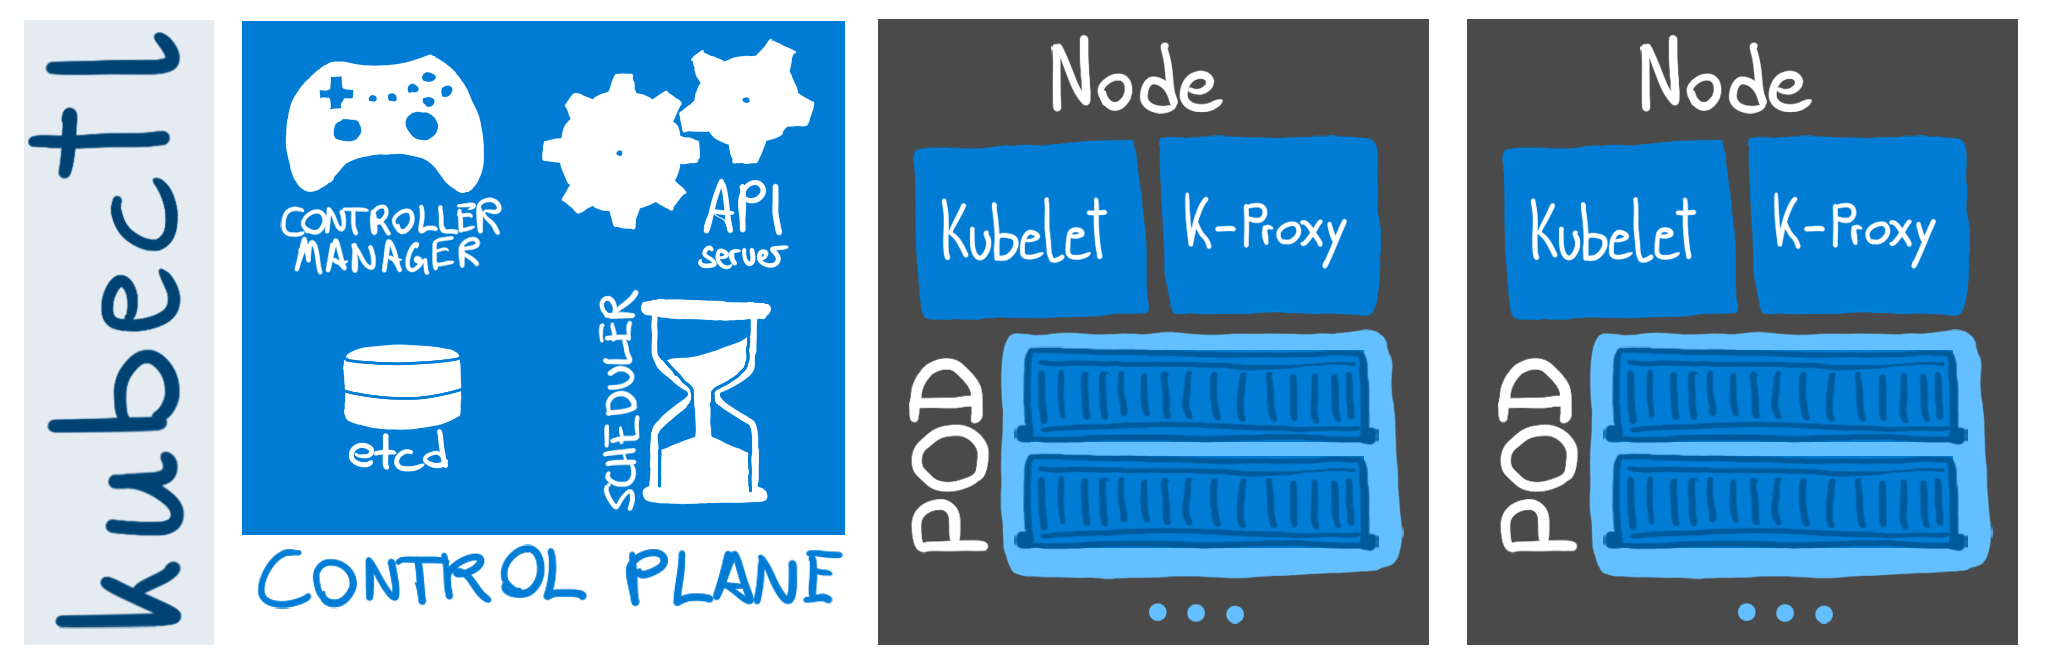
\includegraphics[width=\textwidth]{pics/kubernetes_sketch.png}
\end{frame}

\begin{frame}[fragile]
	\frametitle{Kubernetes objects}
		Just a few should be mentioned here:
		\begin{itemize}
			\item \hervor{Deployment}: packaged application consisting of several containers run in a \hervor{Pod}. Can be replicated for load balancing.
			\item  \hervor{Service}: A connection to an application, "pod-agnostic" for availability
			\item \hervor{Pods}, \hervor{Nodes}, etc. are Kubernetes objects too! Get information about them with
			\begin{lstlisting}
# info for all objects of one type
kubectl get object
kubectl describe object
# info for a specific object
kubectl get object objectname
kubectl describe object objectname
			\end{lstlisting}
		\item \hervor{Control Plane} controls a cluster of \hervor{Nodes}
		\item containers are deployed in \hervor{Pods} on \hervor{Nodes}
			\end{itemize}

\end{frame}

\begin{frame}[fragile]
	\frametitle{Interacting with the cluster: \texttt{kubectl}}
	\begin{block}{\texttt{kubectl}}
	is a CLI tool to send commands to the \hervor{API server} for creating Kubernetes objects.
	\end{block}
	\codi{kubectl} creates objects
	\begin{itemize}
		\item \hervor{imperatively}: Everything explicitly on the command line 
		\item \hervor{declaratively}: with a \hervor{spec} representing the desired state (\codi{.yaml}-file)
	\end{itemize}
	Let the cluster work to realize your spec:
	\begin{lstlisting}
kubectl apply -f kubernetes/greeting-depl-0-1.yaml
kubectl apply -f kubernetes/greeting-depl-0-2.yaml
	\end{lstlisting}
	Declarative way is preferred and more practicable!
\end{frame}

\begin{frame}[fragile]
	\frametitle{Create a greeting app deployment and service}
	\vspace{-.2cm}\begin{columns}
		\column{.5\textwidth}
		\begin{lstlisting}
apiVersion: apps/v1
kind: Deployment
metadata:
  name: greeting-depl
spec:
  selector:
	matchLabels:
	  app: greetingapp
  replicas: 2 # 2 pods of template
  template:
	metadata:
	  labels:
		app: greetingapp
	spec:
	  containers:
	  - name: greet
		image: greeting:0.1
		ports:
		- containerPort: 5000
		\end{lstlisting}
	
		\column{.47\textwidth}
		\textbf{Example:} \codi{kubernetes/greeting-depl-0-1.yaml}
		\begin{lstlisting}
kubectl apply \
	-f greeting-depl-0-1.yaml
# see what just happened
kubectl get deployments
kubectl get pods
kubectl logs podname containername
		\end{lstlisting}

		Make available by creating a \hervor{service}:
		\begin{lstlisting}
kubectl expose deployment \
	greeting-depl \
	--type=NodePort \
	--port 5000
# note the port it gets mapped to
kubectl get services
# run proxy for access on localhost
kubectl proxy
		\end{lstlisting}
	\end{columns}
\end{frame}

\begin{frame}[fragile]
	\frametitle{Update greeting app deployment}

		\textbf{Example:} \codi{kubernetes/greeting-depl-0-2.yaml}
		\begin{itemize}
			\item Updated greeting image version
			\item Added postgres container
		\end{itemize}
		Declare the new spec:
		\begin{lstlisting}
kubectl apply -f greeting-depl-0-2.yaml
		\end{lstlisting}
	\begin{itemize}
		\item Pods are replaced one by one, without the service terminating!
		\item Eventually, you will see the newer greeting app.
		\end{itemize}
		
		Tidy up:
		\begin{lstlisting}
kubectl delete service greeting-depl
kubectl delete deployment greeting-depl
		\end{lstlisting}
		Containers and pods are terminated!
		
	
\end{frame}

\begin{frame}
	\frametitle{Concluding notes}
	
	\begin{itemize}
		\item replicas $>1$: we do not know which of our apps we will get (\hervor{load balancing}, no persistent storage)
		\item persistent storage is possible, here only stateless applications were shown
		\item \textbf{Not mentioned here:} security, encryption, secrets
		\item Docker Desktop users can activate a one-node kubernetes cluster in the settings
		\item Another one-node try-out solution: \myhref{https://minikube.sigs.k8s.io/docs/}{Minikube}
	\end{itemize}

	\begin{block}{Further reading:}
	\begin{itemize}
		\item \myhref{https://kubernetes.io/docs/home/}{Kubernetes documentation}: Includes lots of learning resources and examples.
		\item \myhref{https://training.play-with-kubernetes.com/}{Play with Kubernetes classroom}: Interactive training session giving an overview over concepts.
	\end{itemize}
	
	\end{block}
\end{frame}

\sectionslide{Thank you for participating!}

\end{document}